\documentclass[10pt,a4paper]{book}

\usepackage[utf8]{inputenc}
\usepackage[english]{babel}
\usepackage{amsmath}
\usepackage{amsfonts}
\usepackage{amssymb}
\usepackage{graphicx}
\usepackage{fancyvrb}
\usepackage[parfill]{parskip}
\usepackage[left=3cm,right=3cm,top=3cm,bottom=3cm]{geometry}

\newcommand{\ROOT}{\Verb`ROOT` }
\newcommand{\Judith}{\Verb`Judith` }

\author{Garrin McGoldrick}
\title{Judith Reference Manual}

\begin{document}

\maketitle

\pagenumbering{Roman}
\tableofcontents
\newpage

\pagenumbering{arabic}

\chapter{Introduction}
\label{ch:introduction}

Do read this chapter, it will probably save you some time down the road. This (brief) introduction is meant to explain where you can find what you are seeking in this document, and where you can find information you weren't looking for but probably need.

This document isn't an exhaustive reference, it is instead only a guide describing the organization and general features of \Judith. The exhaustive reference is the source code which is well commented and meant to be very readable (in that way it is self-documenting).

If you aren't an experienced C++ programmer (i.e. you read C++ code, and you write algorithms, but maybe you've never sat down to read a book on it) you should head to appendix \ref{ch:cppprimer}. Even if you are an experience C++ programmer, you might find some useful information there. It will take only 10 minutes of your time and save you hours of head and heart aches. The introduction will be waiting for you to come back, its not going anywhere.

The typical user is expected to have some level of familiarity with C++ and Unix, but may not be well versed in either topic. Some basic information about both subjects will be included in this document to put all readers on equal footing.

\subsubsection*{Navigating the source code}

This document is meant to be used as a sort of map whereby you can look up a topic on which you want more information, and it will indicate where and how it is implemented in the source code.

For the Unix uninitiated, you should know of at least two tools: \Verb`man` and \Verb`grep`. \Verb`man name` will show you the manual entry for the binary called \Verb`name`. \Verb`grep` will allow you to search within a directory for any occurrences of a string of text, allowing for regular expressions. \Verb`man grep` will get you started.

Say you want to find where the method \Verb`getPixX` is implemented. From the program's base directory run: \Verb`grep -rn 'Hit::getPixX(' src/`. Or, better yet, where the error ``plane mask is too small'' is thrown: \Verb`grep -rn 'plane mask is too small' src/`. If any of this seems like a foreign language, you may need to bush up on any or all of: Unix, bash, C++.

\subsubsection*{Finding a topic}

This document and the source code are organized into modules, described in chapter \ref{ch:modules}. The source code is organized in a typical C++ directory structure. Following is an overview of the important parts of the source:

\begin{itemize}
	\item \Verb`include/` : this part of the code serves as documentation since nearly all functions are declared here with a brief description.
	\begin{itemize}
		\item \Verb`module/` : files are grouped by module.
		\begin{itemize}
			\item \Verb`header.h` : the declarations of a particular class or functions within the module.
		\end{itemize}
	\end{itemize}
	\item \Verb`src/` : this is where the code is implemented.
	\begin{itemize}
		\item \Verb`module/` : files are grouped by module.
		\begin{itemize}
			\item \Verb`source.cxx` : the definitions of a particular class or functions within the module.
		\end{itemize}
	\end{itemize}
\end{itemize}

Following is a brief overview of the modules' contents:

\begin{description}
	\item[\Verb`storage`]: memory representation of objects (e.g. \Verb`Hits`), and their input and output.
	\item[\Verb`mechanics`]: description and manipulation of the physical properties of detector and detector systems (e.g. alignment, noise mask).
	\item[\Verb`utils`]: general purpose algorithms used in various parts of the program (e.g. linear fit).
	\item[\Verb`processors`]: classes which process event-by-event information (e.g. clustering).
	\item[\Verb`analyzers`]: classes which combine processors (and other elements) to perform analysis tasks, called on an event-by-event basis (e.g. plotting algorithms).
	\item[\Verb`loopers`]: control structures which loop over a dataset of events (e.g. synchronization loop, event processing loop).
	\item[\Verb`configuration`]: configuration and instantiation of program elements from configuration files.
\end{description}

\subsubsection*{Program gaols}

The following is a vague statement of the goals of \Judith:

\begin{itemize}
	\item Transparent: the main goal is for the program to be transparent to users. It is expected that every use case will differ, and some customization will be desired. For this reason, the program should be easily understood and extended by non-expert-programmers (i.e. physicists).
	\item Fast: this program is expected to be used in testbeam type situations where time is constrained and very valuable. Testbeam users will need to see results quickly so they can react to them in real-time. The time scale for performing tasks should be minutes at most, and preferably seconds.
	\item Simple: this follows from the two previous point. The program should implement simple algorithms which are efficient, easily understood, and easily extended or modified.
	\item Portable (except on Windows, because Windows): the program should be deployable in a variety of contexts. E.g. on a user's laptop which can be carried into different laboratories, on a DAQ desktop controlling some testbeam hardware, on a work computer for analysis. The targeted deployment systems are Linux and Mac.
\end{itemize}

\chapter{Quick start guide}

\chapter{Modules}
\label{ch:modules}

\section{Overview}

The \Judith program is separated into modules which fulfil separate needs. The modules are compiled into separate libraries to facilitate the integration of Judith algorithms into other programs.

An overview of module contents is provided in chapter \ref{ch:introduction} The following lists the inter-dependencies of the modules:

\begin{itemize}
    \item \Verb`storage`: stand-alone module.
    \item \Verb`mechanics`: stand-alone module.
    \item \Verb`utils`: stand-alone module.
    \item \Verb`processors`: depends on \Verb`mechanics`, \Verb`utils`.
    \item \Verb`analyzers`: depends \Verb`processors` and \Verb`utils`.
    \item \Verb`loopers`: depends \Verb`storage`, \Verb`mechanics`, \Verb`processors`, \Verb`analyzers`.
    \item \Verb`configuration`: potentially depends on everything.
\end{itemize}

\section{Storage}

The \Verb`Storage` module contains those classes which describe the event memory---that is the data which is loaded on an event-per-event basis. It also includes functionality which can read/write memory from/to disk in the form of a \ROOT n-tuple.

Note that the in the following sections, a series of members are listed for the storage classes; these are stored in the n-tuples as \ROOT \Verb`TBranch` objects. \textbf{Some storage files may omit certain branches} in which case the values are zeroed on read-back. For example, a pixel detector which doesn't detect a hit ``intensity'' may omit the \Verb`Hit`'s \Verb`value` member when writing output n-tuples.

By convention, member variables prefixed with \Verb`pix` describe distances in pixel space. Variables prefixed with \Verb`pos` describe distances in global space. Pixel space is a local coordinate system defined for each sensor such that $x = 0$ corresponds to the center of the first pixel column and $x = \mathrm{ncols} - 1$ corresponds to the center of the last column where ncols is the number of columns. $y$ describes rows in the same manner.

Event data includes event information (e.g. trigger time), digitized hits recorded by sensors, the grouping of those hits into clusters, the grouping of those clusters into tracks and all associated calculated values (e.g. track slope). Stored event data might not include all this information if the information is not available. E.g. only hit information is stored before they have been made into clusters and tracks.

The \Verb`Event` class provides access to its components which describe the event data and calculated values. This relationship is illustrated in figure \ref{fig:modules_storage_objects}. When data isn't available, null pointers are passed in lieu of the object; e.g. an unclustered hit will return 0 when calling \Verb`getCluster()`.

\begin{figure}[htb]
  \centering
  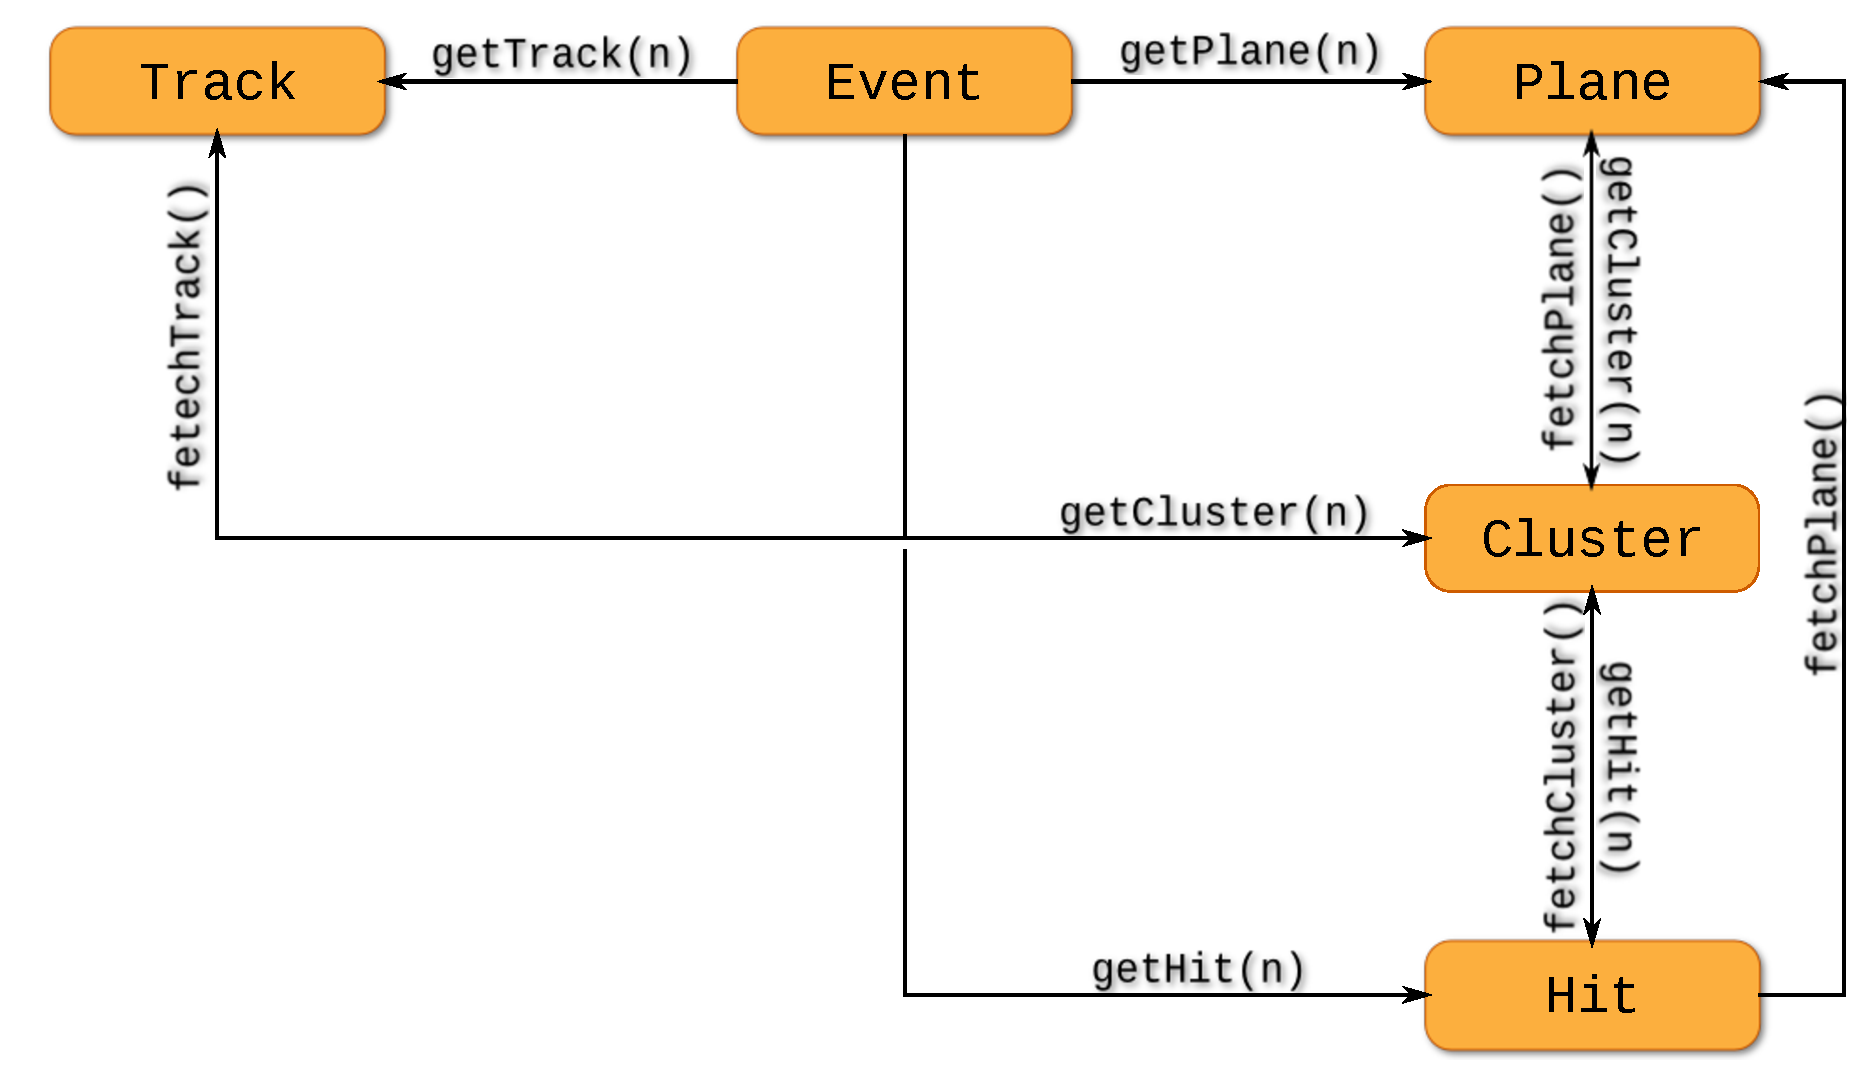
\includegraphics[width=0.7\textwidth]{images/modules_storage_objects.pdf}
  \caption{Association between \protect\Verb`Storage` objects.}
  \label{fig:modules_storage_objects}
\end{figure}

\subsubsection*{Access and ownership}

There are three general manners in which an object's properties can be accessed:

\begin{enumerate}
	\item \Verb`getProperty()`: returns either a value, or a reference to an object. If an object is returned, it is clearly not owned by the user, and is guaranteed to exits.
	\item \Verb`fetchProperty()`: returns a pointer to an object. The returned pointer can be \Verb`NULL` if the property does not exist in the called object. The returned pointer \textbf{is not owned} by the caller, and it is up to the caller to ensure it is not null.
	\item \Verb`getProperty(size_t n)`: returns either a value or a reference to an object, from a list of such values or objects. A corresponding member \Verb`getNumProperties()` will be provided by the called object, and it is up to the caller to ensure \Verb`n` is smaller than this number, otherwise an out of range exception will be thrown.
\end{enumerate}

\subsection{Hit}

The \Verb`Hit` class is the most fundamental unit of each event. It describes the digitized hits recorded by the device sensors. Hits belong to a \Verb`Plane` and optionally to a \Verb`Cluster` which can be accessed as per the calls outlined in figure \ref{fig:modules_storage_objects}.

The \Verb`timing` member is provided to accommodate timing information for individual hits (e.g. offset of hit from trigger). The \Verb`value` member is provided to accomodate a digitzied ``intensity'' value for hits (e.g. time-over-threshold).

A \Verb`masked` member is provided to indicate if this hit is from a masked pixel. Pixel masking can either be applied such that no masked hits are loaded, or such that they are loaded and flagged as masked.

\subsection{Cluster}

The \Verb`Cluster` class represents clusters of hits within one sensor plane which are thought to have been generated by a single particle traversing the sensor. The class contains a list of hits, and some properties calculated from these hits. Clusters belong to a \verb`Plane` and optionally to a \verb`Track` which can be accessed as per the calls outline in figure \ref{fig:modules_storage_objects}.

The center of gravity (COG) and size of the cluster are stored in the \Verb`pix` and \Verb`pixErr` members respectively in pixel coordinates. The same information is stored in the \Verb`pos` and \Verb`posErr` members in global coordinates.

The \Verb`timing` member contains the lowest timing value from hits comprising the cluster, and the \Verb`value` member contains the sum of values of all hits in the cluster.

\subsection{Track}

The \Verb`Track` class represents a series of clusters in different planes which are thought to have been generated by a single particle traversing the planes. The class contains a list of clusters, and some properties calculated from these clusters.

Fundamentally, a track is just a collection of clusters; this collection can be interpreted in many ways by considering multiple scattering, energy loss etc. A linear fit ``interpretation'' is stored as this is the simplest way to get meaningful information from tracks.

The linear fits are stored in the \Verb`slope` and \Verb`origin` members which are expressed in global coordinates (these values can't be represented in a plane's local coordinate system). The \Verb`slopeErr`, \Verb`originErr` and \Verb`covariance` members can be used to estimate the extrapolation uncertainty of a track. Finally, the \Verb`chi2` ($\chi^2$) member allows to quickly assess the validity of the linear description of a track.

\subsection{Plane}

The \Verb`Plane` class is a convenience class which groups \Verb`Cluster`s and \Verb`Hit`s which were recorded in the same sensor plane for a given event.

This class is used to navigate the event data and doesn't serve any other explicit purpose.

\subsection{Event}

The \Verb`Event` class manages all information and objects representing the information for a single triggered event. It provides structured access to the event information through the hierarchy shown in figure \ref{fig:modules_storage_objects}.
 
The \Verb`Event` class owns its constituent objects (\Verb`Hit`, \Verb`Cluster`, \Verb`Plane`, \Verb`Track`). However, the \Verb`StorageIO` class can take ownership of some of its constituents for caching (all but the planes which do not change event-by-event).

The event serves as a centralized repository from where all event information can be obtained, regardless of whether or not that information is accessible in another class (e.g. \Verb`Hit`s and \Verb`Cluster`s are also accessible from the \Verb`Plane` class).

\subsection{StorageIO}

\chapter{Supported data}

\chapter{Configuration files}

\chapter{Writing analysis code}

\chapter{Unit testing}
\label{ch:unittesting}

The \Judith directory structure includes the \Verb`tests` directory. As the name suggests, it is inhabited by tests: small pieces of code which invoke features of \Judith and compare the outcome to what is expected.

Typically, when developing code, a programmer will want to know if a modification or new feature actually works. First it is compiled, then some ad-hock code might be added to the main method to invoke the feature and check its outcome. \Judith's unit testing is simply a way to centralize and formalize this process. It is probably the simplest form of unit testing but should be sufficient and encourage the writing of tests.

Its purpose to twofold:

\begin{enumerate}
	\item Make writing and running test code easier. The programmer need not hack at a larger piece of code to introduce their test, it can be deployed in a stand-alone main. This is then compiled with the latest code and run from a simple script.
	\item The test code doesn't need to be removed after the test is completed. This adds some level of documentation to the project and allows the test to be used over and over again to ensure the feature is not broken with future development.
\end{enumerate}

Following is an outline of the testing procedure when adding a feature to the code:

\begin{itemize}
	\item Develop the feature, and compile the program. Good development will result in most bugs being caught by the compiler.
	\item Open the \Verb`tests/module/tests_filename.cxx` file corresponding to the module file worked on.
	\item Add a test function to the file:\\
		  \Verb`int test_featureToTest()`.
	\item Add the call to that function in the main:\\
		  \Verb`if ((retval = test_featureToTest()) != 0) return retval;`
	\item Write your test code in your test function. The function must return non-zero when a test has failed, stopping the execution of following tests which might rely on the previous one.
	\item From the root project directory, run:\\
		  \Verb`tests/run.sh`
	\item If compilation fails, you can get the full compilation output by the following:
		  \Verb`cd tests/ && make`
\end{itemize}

\appendix

\chapter{C++ primer}
\label{ch:cppprimer}

This appendix is meant to give an overview of the key features of C++ used in \Judith which might not be familiar to casual C++ users. One of the stated goals of \Judith is transparency; for this reason, the written code is meant to be simple and easily accessible. However, for the code to also be efficient and stable, some departure from C-like C++ is required.

The code features which will likely cause the most confusion, and which are discussed herein, are: the standard library, extravagant use of \Verb`const`, references vs. pointers, throwing exceptions.

The concept of inheritance might also be troublesome for some users, but it cannot be summarized without making grave omissions. Thus, if you are not familiar with the object oriented portion of C++ (e.g. if you do not know why a destructor must be \Verb`virutal` in a base class), then you should find an external resource on the topic.

\section{The standard library}

The standard library (STL) provides access to a set of commonly used, highly optimized C++ functionality. If you have a C++ compiler, you almost definitely have access to the STL; thus its use doesn't require the installation of an additional package.

While it is fairly compact (it doesn't introduce a vast amount of functionality), most casual C++ programmers are not familiar with most of its functionality beyond the very simple output stream (\Verb`std::cout`) and dynamic array wrapper (\Verb`std::vector`).

In this section, most STL features used in \Judith are covered. This is not an exhaustive outline of the standard library.

\subsubsection{Containers}

Containers are data structures which hold many different objects of the same type. An array would thus be a container, but not all containers can behave as arrays do.

The \Verb`std::vector` class is appropriate when the container needs to provide random access (i.e. the ability to ask for any element in the container, not just those at the front and/or back) or when iteration speed is crucial.

One of the biggest pitfalls of the \Verb`std::vector` class is that it must re-allocate its entire array to a new memory location when it is expanded beyond a certain size. Thus, continually calling \Verb`std::vector::push_back()` can be very costly.

Following is a list of other common STL containers and their use:

\begin{description}
	\item[\Verb`std::list`]: useful when the container is frequently resized, and when it will usually be iterated only sequentially.
	\item[\Verb`std::stack`]: useful when only the last item in the container needs to be accessed, and when new items are frequently added or removed from the top of the container.
	\item[\Verb`std::map`]: associates a key to each item, so they can be accessed by something other than an index.
	\item[\Verb`std::set`]: ensures there is only ever 1 item of any given value in the container, and provides fast lookup for these items.
\end{description}

Nearly all containers provide an iterator which allows for iteration code which is both highly efficient and agnostic to the underlying container type:

\begin{Verbatim}
for (std::container<Type>::iterator it = variable.begin();
    it != variable.end(); ++it) {
    // do work here
}
\end{Verbatim}

Note the use of \Verb`++it` instead of \Verb`it++`. Use of the latter incrementation operator makes a copy of the object to increment. This is fine for small built-in types (and is probably optimized out by compilers), but not for the more complex \Verb`iterator` type. A \Verb`const_iterator` is available for iterating over \verb`const` declared containers.

\subsection{Algorithms}

The standard library includes many highly optimized and highly useful algorithms in the \Verb`<algorithm>` header. Here are some favourites:

\begin{description}
	\item[\Verb`sort`]: sort a vector (or other random access container).
	\item[\Verb`partial\_sort`]: when only part of the container needs to be sorted, use this function.
	\item[\Verb`nth\_element`]: when only one element needs to be in its sorted position, use this function.
	\item[\Verb`find`]: find the position of a specified value within a container.
	\item[\Verb`min`, \Verb`max`]: return the smaller or larger of two values, makes code a bit more readable when used.
\end{description}

For various situations especially requiring manipulation of containers, there might be even more appropriate (and thus more optimized) functions available.

\section{Use of const}

This and the following section fall into a school of thought when programming C++: compile-time errors are preferable to run-time errors. If you give enough information to the compiler, it can know when you've written code which might try to do something that shouldn't happen. You then get a descriptive one-time error which you must fix.

In contrast, run-time errors are only detected when they arise during execution, and there's no way to control when that will be (unit tests try to detect as many as possible but aren't perfect). They can happen semi-randomly, and they can lay dormant for a long time before exposing themselves in a catastrophic crash just when you're trying to show off your code. While programs exist to help you find these bugs (do \Verb`man gdb` if gdb means nothing to you), their origins can sometimes be very difficult to track down.

The principle of ``least privilege'' helps turn run-time errors into compile-time errors. By making variables only accessible to those pieces of code you explicitly intend to modify those variables, you minimize the risk of inadvertently modifying something you expected to remain fixed.

Better yet, by declaring any variable \Verb`const` whose value shouldn't change during execution, you greatly constrain the ways in which you can break your program. This is best explained with an unoriginal example: say a car object has a getter which returns its door object. Say this door object gets passed around a few methods until one decides it wants to know how the door looks when it is twice as big. The car will not work with the oversized door, but the method in question doesn't know that the door is hinged to a car. Having the getter return a \Verb`const` door will cause a compile-time error when the culprit method is compiled.

To summarize, \textbf{anything which can be declared \Verb`const` should be declared \Verb`const`}. If it is later realized that it should be mutable, it is very easy to remove the \Verb`const` constraint.

\section{Use of references over pointers}

Pointers are initially terrifying to novice C and C++ programmers. Eventually, (surely through some kind of Stockholm Syndrome mechanism), programmers learn to love pointers and cherish them as the answer to all woes. But eventually, given enough bad experiences, it becomes clear that \textbf{pointers are evil} when misused.

Borrowing from the previous section, pointers tend to cause run-time errors when handled inappropriately, or introduce overhead in order to be handled appropriately.

Pointers definitely have their uses, but a casual C++ programmer might not realize that most uses for pointers can be achieved using references, only with less risk of incurring run-time errors. This is especially true of C++ programmers who learned C++ in tandem with \ROOT which attempts to hide the inherent issues relating to pointers (often resulting in stack traces).

It's worth noting that references aren't completely immune to errors; it is possible to make invalid references, but you either need to try pretty hard (e.g. \Verb`int* pi = 0; int& ri = *pi;`), or the compiler will emit a warning.

Following is a summary of issues that arise when using pointers but not when using references.:

\begin{itemize}
	\item Dereferencing a null pointer: null pointers are often passed to indicate that the underlying data doesn't exist. The user might try to use the pointer without checking if it is null, especially when the pointer \emph{should} have been valid.
	\item Overloaded operators: pointers are essentially integers. Thus, mistakenly writing something like \Verb`pointer++` instead of \Verb`pointer->value++` will be syntactically correct but will cause a run-time crash if \Verb`pointer` is accessed again (unless another object of the same type exist right beside it in memory).
	\item Ownership: when an object returns a pointer, as in \Verb` calledObject->getMemberObject()`, who is responsible for freeing the member object? And what of \Verb`calledObject->newObject()`? Often, the called object source must be read to be sure it is correctly used.
\end{itemize}

References are equally well suited for passing complex objects without copying their contents, they can be used with forward declarations, and they can even have default arguments in argument lists (e.g. \Verb`void function(const std::string& arg="default")` is valid).

Pointers are still better suited for storing objects in containers (\Verb`std::vector<Type&>` is not allowed), and for passing around objects which might not exist. They generally solve the problem of needing a place-holder for an object, which is not bound to a particular object or any object at all.

To summarize, \textbf{if a pointer can be replaced by a reference, it probably should be}.

\section{Throwing exceptions}

Exceptions are another very useful feature which is often overlooked by casual C++ programmers. It allows for any piece of code to stop the process execution with an error message. Better yet, it allows for any piece of code lower in the stack to try to fix the error and prevent the process from exiting.

They are a much more convenient way of indicating a function encountered an error than by returning negative integers. The discussion of how inheritance allows for complex decision making in catching exceptions is not appropriate for an appendix. But suffice to say, returning negative integers is ambiguous at best, and simply annoying in most cases: every function below the one returning the integer must check for a return code and keep propagating it. Then the value needs to be checked against some list of error codes.

Throwing an exception is as simple as \Verb`throw "Something went wrong"` although a better practice would be \Verb`throw std::runtime_error("Something went wrong");`. The exception will propagate down the call tree all the way to the operating system which will terminate the process, unless some code in the call tree tries to catch the exception. The message from the second version will likely be printed regardless of whether or not the exception is handled by the program.

\end{document}

